\section{Durchführung}
\label{sec:Durchführung}
In diesem Versuch sollen unteranderem Emissions- und Absorbtionsspektren untersucht werden. Dazu werden vorbereiten 
zu diesem Versuch die Theoriewerte der im \autoref{subsec:Versuchsdurchführung} erwähnten Messgrößen recherchiert.
\subsection{Vorbereitungsaufgaben}
\label{subsec:vorbereitung}
Da das Emissionsspektrum von Kupfer untersucht werden soll, werden zunächst die hierfür nötigen Theoriewerte bestimmt.
Bei Kupfer liegt die $\symup{K}_\alpha$-Linie bei $\qty{8}{\kilo\electronvolt}$. Daraus kann dann der Bragg-Winkel $\Theta_{\symup{K}} = \qty{22.66}{\degree}$. 
Die $\symup{Cu}\text{-}\symup{K}_{\beta}$-Linie liegt bei $\qty{8.95}{\kilo\electronvolt}$ mit einem Bragg-Winkel von $\Theta_{\symup{K}} = \qty{20.14}{\degree}$.
Nun werden für die fünf Abschirmstoffe die nötigen Theoriewerte bestimmt. Dabei muss auch der Bragg-Winkel bestimmt werden, da man seine Messung so zeitlich optimieren kann.
\begin{table}
    \centering
    \caption{In dieser Tabelle werden die Theoriewerte für die Untesuchung der Abschirmungskonstante dargestellt. Z beschriebt die Ordnungszahl, 
    $E_{\symup{K}}^{\symup{Lit}}$ den Literaturwert der Energie der $K_\alpha$-Linie, $\Theta_{\symup{K}}^{\symup{Lit}}$ den Literaturwert des Bragg-Winkels der $K_\alpha$-Linie
    und $\sigma_{\symup{K}}$ die Abschirmungskonstante eines Materials zur $K_\alpha$-Linie. WINKEL NOCH VON LUKAS NEHMEN UND EVTL N SINNVOLLES NACHSCHLAGWERK REINBALLERN DIGGGGGGGAAAAAAAAAAAAAAAAAAAAAAAAAAAAAAAAAAAAAA}
    \label{tab:vorbereitung}
    \begin{tabular}{c c S S S}
        \toprule
         & Z & {$E_{\symup{K}}^{\symup{Lit}} \mathbin{/} \unit{\kilo\electronvolt}$} & {$\Theta_{\symup{K}}^{\symup{Lit}} \mathbin{/} \unit{\degree}$} & {$\sigma_{\symup{K}}$} \\
        \midrule
        Zn & 30 &  9.65 & 18.60 & 3.56 \\
        Ga & 31 & 10.37 & 17.29 & 3.61 \\
        Ge & 32 & 11.10 & 16.20 & 3.68 \\
        Br & 35 & 13.47 & 13.23 & 3.85 \\
        Rb & 37 & 15.20 & 11.70 & 3.94 \\
        Sr & 38 & 16.10 & 11.04 & 4.00 \\
        Zr & 40 & 17.99 &  9.86 & 4.10 \\
    \bottomrule
    \end{tabular}
\end{table}
\subsection{Versuchsaufbau}
\label{subsec:Versuchsaufbau}
Für diesen Versuch wird eine Kupfer-Röntgenröhre, ein LiF-Kristal, ein Geiger-Müller-Zählrohr und fünf Abschirmproben verschiedener Elemente. 
Die Kupfer-Röntgenröhre, der LiF-Kristal und das Geiger-Müller-Zählrohr sind in einer geschlossenen Vorrichtung eingebaut. Diese ist in \autoref{fig:aufbau} zu sehen.
\begin{figure}
    \centering
    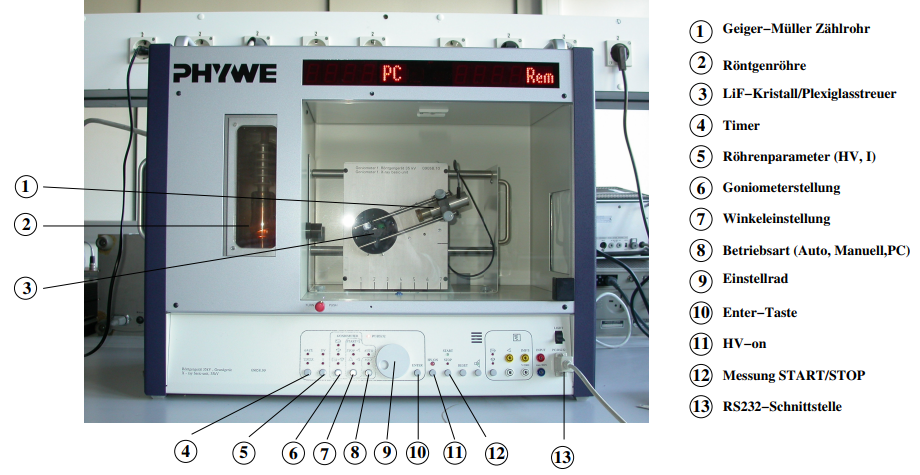
\includegraphics[width = \textwidth]{content/aufbauskizze.PNG}
    \caption{Aufbau der Kupfer-Röntgenröhre, des LiF-Kristals und des Geiger-Müller-Zählrohrs in einer Vorrichtung. \cite{v602}}
    \label{fig:aufbau}
\end{figure}
\subsection{Versuchsdurchführung}
\label{subsec:versuchsdurchführung}
Zu Beginn werden die Apparatur, welche in \autoref{fig:aufbau} zu sehen ist, und der Computer angeschaltet. Auf dem Computer wird das Programm \textit{measure} gestartet.
Dann wird in der oberen Leiste unter dem Menüpunkt \textit{Messgerät} \textit{Röntgengerät} ausgewählt. Nun erscheint ein Einstellungsmenü für das Röntgengerät.
Zuerst wird die Braggbedingung überprüft. Dazu soll der LiF-Kristall in einem Winkel von $\qty{14}{\degree}$ eingestellt. Dies geschieht in dem Einstellungsmenü. Im selben 
Menü wird für das \textit{GMZ}(hier und im folgendem Geiger-Müller-Zählrohr) eine Winkelspanne von $\qty{26}{\degree}$ bis $\qty{30}{\degree}$ eingestellt. Der Winkelzuwachs
wird auf $\qty{0.1}{\degree}$ festgelegt. Es soll für jeden Winkel die Intensität gemessen werden. Es wird eine Integrationzeit von $\Delta t = \qty{5}{\second}$ eingegeben.
Es wird der Winkel mit der maximalen Intensität ermittelt und dann mit dem Theoriewert, welcher aus der Braggbedingung vorhergesagt wird, verglichen.
Darauf hin wird das Emissionsspektrum einer Cu-Röntgenröhre untersucht. Dazu wird zuerst in \textit{measure} der \textit{2:1 Koppelmodus} aktiviert. Für die erste Messung 
wird der Winkelbereich von $\qty{4}{\degree}$ bis $\qty{26}{\degree}$ eingestellt. Der Winkelzuwachs wird auf $\qty{0.2}{\degree}$ gestellt und die Integrationzeit bleibt 
unverändert. Es wird erneut die Intensität gemessen. Nach dieser Messung entsteht eine Graphik, welcher die $\symup{K}_\alpha$- und $\symup{K}_\beta$-Linien entnommen werden
können. Anhand dieser Graphik wird nun ein möglichst kleine Winkelbereich um die beiden Peaks gewählt. Mit diesem Winkelbereich und einem Winkelzuwachs von
$\qty{0.1}{\degree}$ wird erneut die Intensität gemessen, sodass ein Detailspektrum dargestellt wird. 
Zuletzt wird das Absorptionsspektrum untersucht. Dazu wird zuerst ein Zinkabsorber vor dem \textit{GMZ} befestigt. Im Programm \textit{measure} wird ein Winkelzuwachs
von $\qty{0.1}{\degree}$ und eine Integrationszeit von $\Delta t = \qty{20}{\second}$ eingestellt. Da mit dieser Integrationszeit eine Messung über einen großen 
Winkelbereich sehr lange dauert wird ein hinreichend großer, jedoch minimaler, Winkelbereich gewählt. Dieser wird anhand der Tabelle \ref{tab:vorbereitung} in einem Intervall
um den erwarteten Wert gewählt. Diese Prozedur wird für insgesamt fünf der sieben Elemente in der Tabelle \ref{tab:vorbereitung} gemacht. 
